\section{Viola-Jones algoritam}

Prije velikog razvoja konvolucijskih neuronskih mreža, Paul Viola i Michael Jones su 2001. godine u svom radu \citep{ViolaJones} objavili svoj algoritam koji je tada bio prvi algoritam koji je omogućavao detekciju lica u stvarnom vremenu. Iako se može trenirati i na drugim domenama, algoritam je najpoznatiji po detekciji lica pa će na toj domeni ovdje biti i opisan.

Naravno, algoritam treba puno pozitivnih (slike lica) i negativnih primjera (slike bez lica). Iz tih slika potrebno je izvući značajke prema kojima će kasnije biti moguće odrediti (detektirati) lice. Za ekstraciju značajki koriste se Haarove značajke.

\begin{figure}[htb]
	\centering
	\begin{subfigure}[b]{0.4\linewidth}
		
\includegraphics[width=\linewidth]{img/EdgeFeatures.png}
		\caption{Značajke rubova}
		\label{img:haar-features1}
	\end{subfigure}
	\begin{subfigure}[b]{0.4\linewidth}
		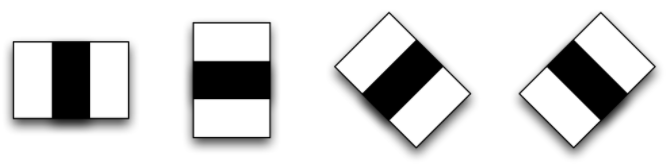
\includegraphics[width=\linewidth]{img/LineFeatures.png}
		\caption{Linijske značajke}
		\label{img:haar-features2}
	\end{subfigure}
	\begin{subfigure}[b]{0.4\linewidth}
		
\includegraphics[width=\linewidth]{img/DiagonalFeatures.png}
		\caption{Dijagonalne značajke}
		\label{img:haar-features3}
	\end{subfigure}
	\begin{subfigure}[b]{0.4\linewidth}
		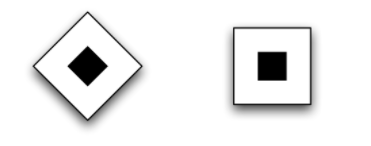
\includegraphics[width=\linewidth]{img/CenterSorround.png}
		\caption{Radijalne značajke}
		\label{img:haar-features4}
	\end{subfigure}
	\caption{Haarove značajke}
	\label{img:haar-features}
\end{figure}

Haarove značajke računaju se na temelju razlike u intenzitetu piksela. Primjerice, ako su vrijednosti piksela u rasponu od 0 (bijeli piksel) do 1 (crni piksel), svi pikseli koji imaju vrijednost veću do 0.5 smatraju se tamnim, a svi pikseli koji imaju vrijednost manju od 0.5 smatraju se svijetlima. Na slici \ref{img:haar-features} prikazane su 4 kategorije Haarovih značajki. Dakle, kako bi bilo moguće odrediti gdje se na slici nalazi (i ako se nalazi) neka od značajki, slika se dijeli na manja područja te se na svakom od tih područja traže Haarove značajke. Naravno, značajke se skaliraju i rotiraju kako bi se pronašli svi dijelovi slike koji zadovoljavaju uvjete značajki. Zatim se odredi gledano područje, kao što to prikazuje slika \ref{img:haar-calc}, te se računaju vrijednosti za Haarove značajke po formuli:
\[
\Delta = dark - white = \frac{1}{n}\sum_{}^{n}I_{dark}(x) - \frac{1}{n}\sum_{}^{n}I_{light}(x)
\]

\begin{figure}[htb]
	\centering
	\begin{subfigure}[b]{0.4\linewidth}
		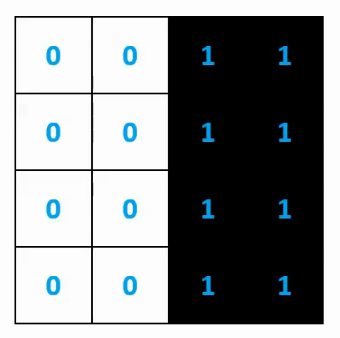
\includegraphics[width=\linewidth]{img/IdealHaarFeatures.png}
		\caption{Idealne vrijednosti piksela}
		\label{img:haar-ideal-features}
	\end{subfigure}
	\begin{subfigure}[b]{0.4\linewidth}
		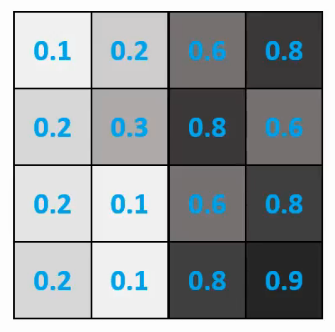
\includegraphics[width=\linewidth]{img/RealHaarFeatures.png}
		\caption{Stvarne vrijednosti piksela}
		\label{img:haar-real-features}
	\end{subfigure}
	\caption{Izračun za linijske Haarove značajke}
	\label{img:haar-calc}
\end{figure}


Slika \ref{img:haar-features1} prikazuje Haarove značajke rubova. Neke od primjena tih značajki su detekcija obrva, gornje/donje usne i zubi. Slika \ref{img:haar-features2} prikazuje linijske Haarove značajke koje služe za detekciju nosa, usta, očiju itd. Nadalje, slika \ref{img:haar-features3} prikazuje dijagonalne Haarove značajke koje se koriste u detekciji složenijih karakteristika. Recimo, ako se lice na slici smije, rubovi usana se uvuku u obraze te su tada slabije osvjetljeni. Tako zajedno sa okom na istoj strani lica tvore tamnije zone, dok obraz i nos čine svijetlija područja. Zadnja skupina Haarovih značajki su radijalne Haarove značajke koje prikazuje slika \ref{img:haar-features4}. Te se značajke koriste u detekciji zjenica, rubova usana i sl. Dakle, Haarove značajke mogu se shvatiti kao preteča konvolucijskih jezgri. Slika \ref{img:haar-image} prikazuje neke od haarovih značajki detektiranih na slici.

\begin{figure}[htb]
	\centering
	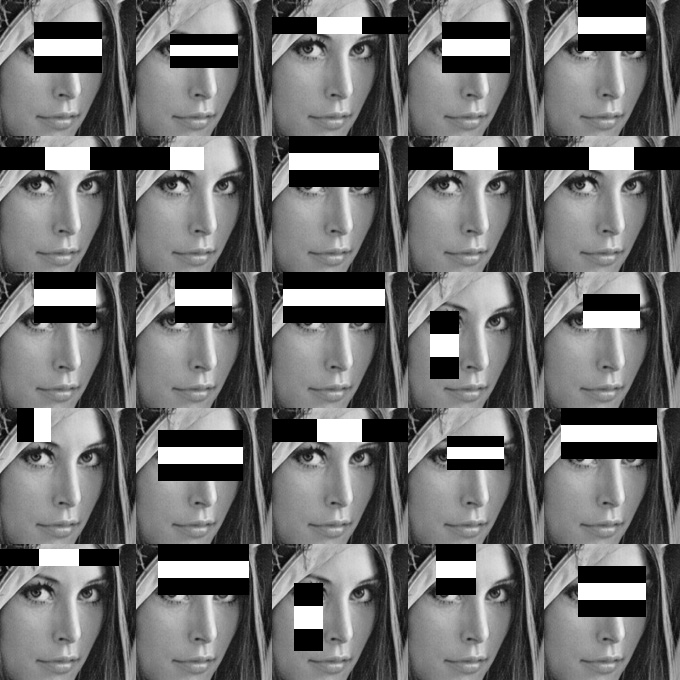
\includegraphics[width=12cm]{img/Haar3.jpg}
	\caption{Neke od Haarovih značajki pronađenih na slici}
	\label{img:haar-image}
\end{figure}

Ovaj proces je dosta spor i neefikasan jer se na ovakav način dođe do više od 160000 različitih značajki. Očito je da, ovisno o domeni, neke od značajki odgovaraju više od drugih, no javlja se pitanje kako odabrati najbolje značajke? Odgovor na ovo pitanje je Adaboost algoritam. Adaboost (skraćeno od \textit{engl. Adaptive Boosting}) je algoritam osmišljen 2003. godine koji kombinira izlaze iz ostalih, "slabijih" kalsifikatora, te njihovom težinskom sumom dolazi do optimuma algoritma. Adaboost zapravo uči i optimizira težine za svaki od klasifikatora.

\begin{figure}[htb]
	\centering
	
\includegraphics[width=\linewidth]{img/Viola-Jones.png}
	\caption{Viola-Jones algoritam}
	\label{img:viola-jones}
\end{figure}

Autori su došli do zaključka da je čak sa samo 200 značajki moguće postići točnost pronalaženja lica od 95\%. Konačne postavke algoritma iz rada \citep{ViolaJones} sadržavale su oko 6000 značajki. Kako bi optmimizirali ovaj složeni proces i izbjegli primjenu svih 6000 značajki na svaku sliku, Viola i Jones odlučili su napraviti strukturu kaskada značajki u kojoj svaka iduća razina ima sve složenije Haarove značajke. Kao što je označeno na slici \ref{img:haar-cascades}, svaka razina ima mogućnost odbaciti sliku ukoliko ne nađe značajke svoje razine na slici. Tako se dijelovi slike koji ne prikazuju lice odbacuju te se oslobađaju računalni resursi za procesiranje slika na kojima se nalazi lice. Autori navode da je prosjek značajki evaluiranih po slici oko 10.

\begin{figure}[htb]
	\centering
	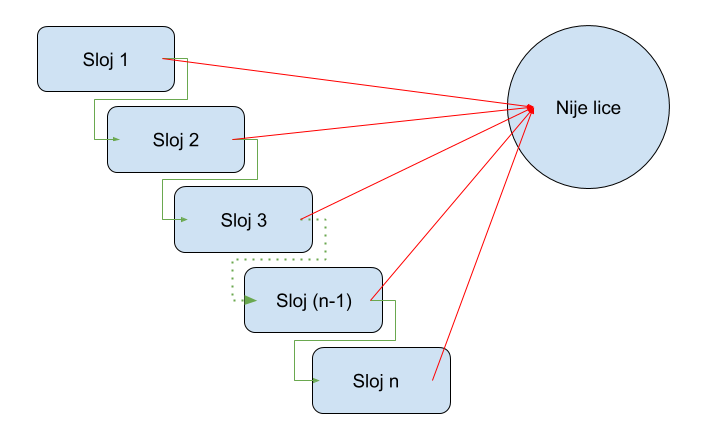
\includegraphics[width=\linewidth]{img/HaarCascades.png}
	\caption{Kaskada Haarovih značajki}
	\label{img:haar-cascades}
\end{figure}

\begin{figure}[htb]
	\centering
	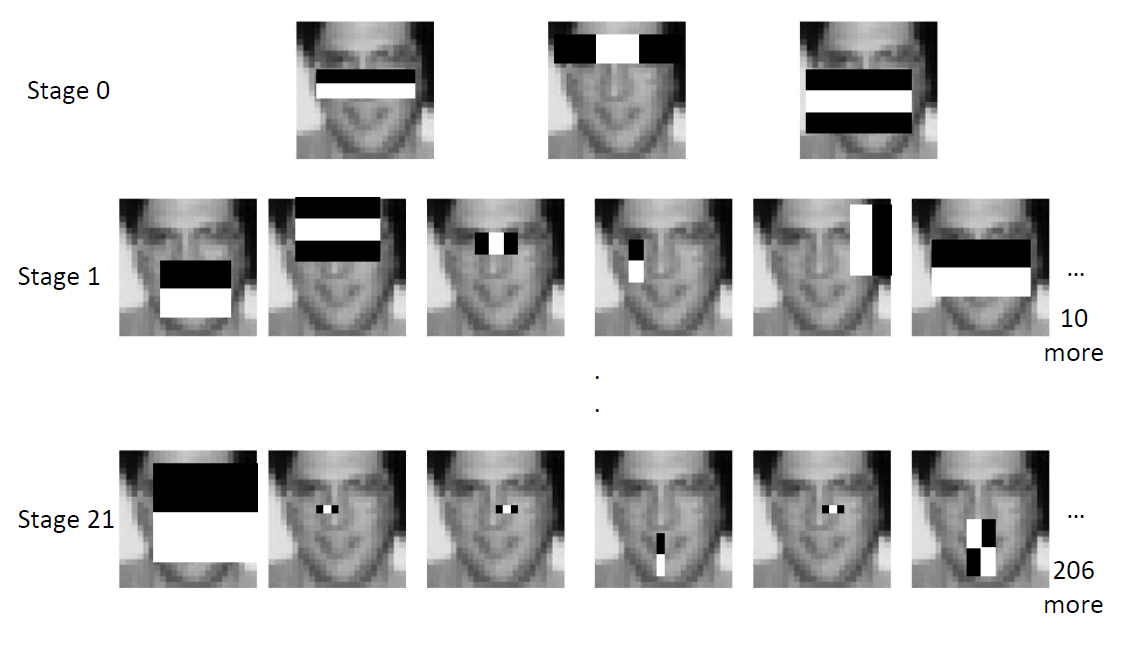
\includegraphics[width=\linewidth]{img/haar2.jpg}
	\caption{Dijelovi Haarovih značajki pronađeni na različitim razinama kaskada}
	\label{img:haar-cascade-layers}
\end{figure}

Rezultati ovih slabijih klasifikatora kombiniraju se u konačni klasifikator koji odlučuje nalazi li se lice na slici. 

Viola-Jones algoritam je svojedobno bio vrlo popularan algoritam jer nudi vrlo pouzdane rezultate, obradu u stvarnom vremenu i invarijantnost na skaliranje. No, isto tako, ima i nekoliko nedostataka kao što su netolerantnost na rotaciju, osjetljivost na osvjetljenje objekata na slici i sl. Činjenica da se još i danas koristi govori dovoljno o kvaliteti i važnosti ovog algoritma.
